% Build from documentation/: latexmk -pdf -interaction=nonstopmode -halt-on-error sparse_autoencoder_models.tex
\documentclass[11pt,a4paper]{article}
\usepackage[T1]{fontenc}
\usepackage[utf8]{inputenc}
\usepackage{lmodern,microtype}
\usepackage[margin=24mm]{geometry}
\usepackage{amsmath,amssymb,mathtools,bm}
\usepackage{booktabs,tabularx,array,longtable}
\usepackage{graphicx,xcolor,tikz,pgfplots}
\usetikzlibrary{arrows.meta,positioning}
\pgfplotsset{compat=1.18}
\usepackage[numbers,sort&compress]{natbib}
\usepackage{enumitem,listings,fancyhdr}
\usepackage[breaklinks,colorlinks,linkcolor=blue!45!black,citecolor=blue!45!black,urlcolor=blue!45!black]{hyperref}
\usepackage{bookmark}
\definecolor{ink}{RGB}{29,48,66}
\definecolor{accent}{RGB}{0,112,128}
\definecolor{paperblue}{RGB}{236,245,248}
\hypersetup{pdftitle={Sparse Autoencoder Baselines for Audio Representation},pdfauthor={LRAC research project}}
\pagestyle{fancy}
\fancyhf{}
\fancyhead[L]{\small\textcolor{ink}{LRAC / Audio representation baselines}}
\fancyhead[R]{\small 28 October 2026}
\fancyfoot[C]{\thepage}
\setlength{\headheight}{14pt}
\setlength{\parindent}{0pt}
\setlength{\parskip}{5pt}
\setlist{nosep,leftmargin=*}
\renewcommand{\arraystretch}{1.16}
\newcolumntype{Y}{>{\raggedright\arraybackslash}X}
\newcommand{\R}{\mathbb{R}}
\newcommand{\norm}[1]{\left\lVert#1\right\rVert}
\newcommand{\code}[1]{\texttt{\small\detokenize{#1}}}
\newcommand{\topk}{\mathcal{H}_k}
\lstset{basicstyle=\ttfamily\footnotesize,breaklines=true,columns=fullflexible,keepspaces=true,frame=single,rulecolor=\color{black!15},backgroundcolor=\color{black!2},aboveskip=8pt,belowskip=8pt}
\title{\textcolor{ink}{Sparse Autoencoder Baselines\\for Audio Representation}\\[6pt]\large Mathematical formulation, exact architecture, training protocol,\\and measured comparison of three models}
\author{LRAC research project}
\date{28 October 2026}
\begin{document}
\maketitle
\begin{abstract}
The research objective is to discover a representation that reconstructs a particular audio signal using as few retained scalar values as possible, without requiring a named transform or interpretable feature labels. This report specifies the first controlled experiment: a sparse nonlinear convolutional autoencoder, its dense-trained nonlinear control, and a sparse affine analysis--synthesis control. All three contain 1,002,369 trainable parameters and were trained for 20,000 updates on the same speaker-balanced ten-hour subset of LibriSpeech. The affine control leads the 200-utterance development comparison and the full 2,620-utterance held-out test. Architecture review also identifies hidden compression to half the input dimensionality before the final latent projection. This is an achieved sparsity--distortion comparison within a restricted model family, not a certificate of the sparsest possible representation, a lossless transform, or a measured audio bitrate. The report connects architecture and objectives to the implementation, reports the observed results, and identifies the remaining research questions.
\end{abstract}
\vspace{4pt}
\colorbox{paperblue}{\parbox{\dimexpr\linewidth-2\fboxsep\relax}{\textbf{Experimental status.} Training and held-out evaluation are complete for three models. Development results use 200 utterances from 40 \code{dev-clean} speakers and also selected checkpoints. The held-out comparison uses all 2,620 \code{test-clean} utterances from 40 different speakers, with frozen checkpoints and budgets. This revision also identifies the shared hidden dimensional bottleneck before sparsification.}}
\newpage
{\small\setlength{\parskip}{0pt}\tableofcontents}
\newpage

\section{Research question and scope}
For an audio vector $x\in\R^N$, the desired system produces a short representation from which a decoder reconstructs $x$ to a specified accuracy. It need not recognize a Fourier transform, label phonemes, or explain the meaning of a feature. A distortion-dependent ideal, after fixing an admissible decoder family $\mathcal G$, is
\begin{equation}
 K^*_{\mathcal G}(x,\varepsilon)=\min_{g\in\mathcal G,\,z}\norm{z}_0
 \quad\text{subject to}\quad d(x,g(z))\leq\varepsilon.
 \label{eq:ideal}
\end{equation}
Here $\norm{z}_0$ counts nonzero scalar coordinates, not time frames, channels, or semantic features. Different distortion measures can give different answers.

Equation~\eqref{eq:ideal} is meaningful only if the decoder, its admissible dependence on the sample, precision, and side information are specified. An unconstrained per-sample decoder can simply memorize $x$ and reconstruct it from an empty code. Even an orthogonal transform chosen separately for $x\ne0$ can map it to $(\norm{x}_2,0,\ldots,0)$; the transform then contains its direction. These are elementary counterexamples, not proposed solutions. Description length offers a complementary accounting perspective~\cite{rissanen1978}.

For this baseline, one encoder and one decoder are learned from training recordings and then frozen. The code and its support change for each input; network weights do not. For a fixed decoder $g_\theta$, the encoder is an amortized proposal for a sparse code, rather than a solver that proves the minimum:
\begin{equation}
 z_k(x)=\topk(f_\phi(x)),\qquad \widehat x_k=g_\theta(z_k(x)).
 \label{eq:baseline}
\end{equation}
We measure the attainable pairs $(\norm{z_k(x)}_0,d(x,\widehat x_k))$. If a code satisfies a tolerance, its support is an \emph{upper bound} on the best support attainable with that decoder and the same numerical conventions. A failed encoder proposal gives no lower bound on other possible codes.

\subsection{Why these three models?}
The comparison changes two concrete choices while preserving the data, training budget, channel counts, parameter count, and evaluation code:
\begin{center}
\begin{tabularx}{\linewidth}{lYYY}
\toprule
ID & Encoder/decoder activation & Training support & Question \\
\midrule
S-NL & Leaky ReLU & Seven sampled fractions & Can reconstruction training organize values to survive severe pruning? \\
D-NL & Leaky ReLU & All values & What changes if sparsity is imposed only after dense training? \\
S-AF & Identity & Seven sampled fractions & Does the nonlinear network help relative to an affine analysis--synthesis map? \\
\bottomrule
\end{tabularx}
\end{center}
The sparse autoencoder follows the hard activation-selection idea of $k$-sparse autoencoders~\cite{makhzani2014}, adapted here to signed convolutional audio codes, magnitude ranking, and multiple whole-recording budgets. It is not an exact reproduction of that paper's network or experiments. The residual connections follow the general residual-learning construction~\cite{he2016}; the specific one-dimensional architecture below is this project's baseline design.

\section{Shared representation and architecture}
\subsection{Inputs, lengths, and dense code capacity}
Inputs are decoded mono waveforms at $F_s=16{,}000$ Hz, represented as float32 tensors of shape $(B,1,N_{\max})$, together with valid lengths $N_i$. There is no per-recording gain normalization, transcript input, speaker embedding, or target-dependent information supplied to the decoder.

Each valid waveform is right-padded to
\begin{equation}
 \overline N_i=256\left\lceil\frac{N_i}{256}\right\rceil,\quad
 T_i=\left\lceil\frac{N_i}{256}\right\rceil,\quad
 C=256,\quad M_i=C T_i.
 \label{eq:capacity}
\end{equation}
The encoder returns $U_i\in\R^{T_i\times256}$. Flattening gives $u_i\in\R^{M_i}$. For a two-second training crop, $N=32{,}000$, $T=125$, and $M=32{,}000$: the \emph{final dense code} has the same number of scalar slots as the waveform. For other lengths, $M$ can be slightly larger than $N$ because of the last partially occupied time step. This slot count does not imply an information-preserving dense encoder: the preceding hidden layer is smaller, as detailed below.

Batch padding is excluded. The implementation encodes equal-valid-length items together so that a longer item in the same batch cannot alter a shorter item's boundary activations. The coefficient mask is
\begin{equation}
 V_i[t,c]=\mathbf 1\{256t<N_i\},\qquad c=0,\ldots,255.
\end{equation}
All 256 channels in a partially occupied final step count toward valid capacity. They are not silently discarded from sparsity accounting.

\subsection{Layer definitions}
Write $\mathcal C^{a\to b}_{q,s,p}$ for a biased 1D convolution with kernel length $q$, stride $s$, and padding $p$. Its cross-correlation convention is
\begin{equation}
 [\mathcal C(h)]_{b,t}=b_b+\sum_{a=1}^{C_{\rm in}}\sum_{j=0}^{q-1}
 W_{b,a,j}\,h_{a,st+j-p},
\end{equation}
with zero values outside the valid padded extent. Let $\mathcal T^{a\to b}_{9,4,4,3}$ denote the corresponding transposed-convolution layer with output padding 3. For input length $L$, its output length is
\begin{equation}
 (L-1)4-2(4)+(9-1)+3+1=4L.
\end{equation}
Transposed convolution is a learned synthesis operation; it is not assumed to invert the encoder convolution.

For S-NL and D-NL,
\begin{equation}
 \sigma(v)=\begin{cases}v,&v\geq0,\\0.2v,&v<0.\end{cases}
 \qquad
 \mathcal R_c(h)=h+\mathcal C^{c\to c}_{3,1,1}\!\left(
 \sigma\!\left(\mathcal C^{c\to c}_{3,1,1}(h)\right)\right).
 \label{eq:residual}
\end{equation}
The two convolutions inside $\mathcal R_c$ have separate parameters. There is no additional activation after the residual sum. In S-AF, every occurrence of $\sigma$ is replaced by the identity, including the activation inside each residual block.

\begin{figure}[htbp]
\centering
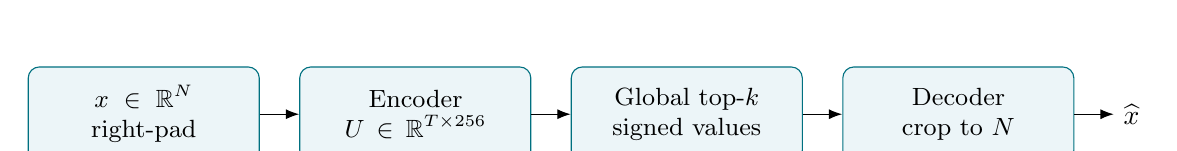
\begin{tikzpicture}[node distance=5mm,box/.style={draw=accent,rounded corners,fill=paperblue,minimum height=12mm,text width=27mm,align=center,font=\small},>=Latex]
\node[box] (x) {$x\in\R^N$\\right-pad};
\node[box,right=of x] (e) {Encoder\\$U\in\R^{T\times256}$};
\node[box,right=of e] (h) {Global top-$k$\\signed values};
\node[box,right=of h] (d) {Decoder\\crop to $N$};
\node[right=5mm of d] (y) {$\widehat x$};
\draw[->] (x)--(e);\draw[->] (e)--(h);\draw[->] (h)--(d);\draw[->] (d)--(y);
\end{tikzpicture}
\caption{The three models share this path. No waveform bypass is available to the decoder. Support positions, the sparse values, the shared model, and length metadata are required for reconstruction.}
\end{figure}

\subsection{Encoder: exact operation order}
For channel sequence $(1,32,64,128,128)$, stage $j$ is
\begin{equation}
 h_j=\mathcal R_{c_j}\!\left(\sigma\!\left(\mathcal C^{c_{j-1}\to c_j}_{9,4,4}(h_{j-1})\right)\right),
 \qquad h_0=x_{\rm padded},\quad j=1,\ldots,4.
\end{equation}
A final biased $1\times1$ convolution maps 128 channels to 256. The result is transposed from $(B,C,T)$ to $(B,T,C)$ for support selection. There is no latent positivity constraint.

\begin{table}[htbp]
\centering\small
\begin{tabular}{llrr}
\toprule
Stage & Operations & Output $C\times L$ for 2 s & Parameters \\
\midrule
E1 & Conv $1\to32$; $\sigma$; $\mathcal R_{32}$ & $32\times8000$ & 6,528 \\
E2 & Conv $32\to64$; $\sigma$; $\mathcal R_{64}$ & $64\times2000$ & 43,200 \\
E3 & Conv $64\to128$; $\sigma$; $\mathcal R_{128}$ & $128\times500$ & 172,416 \\
E4 & Conv $128\to128$; $\sigma$; $\mathcal R_{128}$ & $128\times125$ & 246,144 \\
Latent & Conv $128\to256$, kernel 1 & $256\times125$ & 33,024 \\
\midrule
Encoder total &&& 501,312 \\
\bottomrule
\end{tabular}
\caption{Encoder geometry and trainable counts, including biases. All non-$1\times1$ stage convolutions use kernel 9, stride 4, padding 4. Residual convolutions use kernel 3, stride 1, padding 1.}
\label{tab:encoder}
\end{table}

The temporal hop is $4^4=256$ samples, or 16 ms. The maximum receptive field of a dense encoder coordinate is 2,041 samples, approximately 127.6 ms. To verify this, start with receptive field $r=1$ and jump $j=1$. At each stage add $8j$ for the stride-4 convolution, set $j\leftarrow4j$, then add $4j$ for the two residual convolutions. Thus candidate values are locally computed, although support selection compares candidates across the whole recording.

\paragraph{Hidden compression before sparsification.}
E4 produces only $H=128T=16{,}000$ values for a two-second crop, before the final $128\to256$ projection expands them to $M=32{,}000$ slots. The decoder's first projection similarly reduces 256 channels to 128. All three baselines therefore have a hidden dimensional bottleneck even at full support. The earlier interpretation that only top-$k$ supplies a bottleneck was incomplete; this revision makes the hidden compression explicit.

For S-AF at a fixed length, the effective analysis and synthesis operators in Eq.~\eqref{eq:affine} obey
\begin{equation}
 \operatorname{rank}(B)\leq H,\qquad \operatorname{rank}(A)\leq H.
\end{equation}
At $N=32{,}000$, $H=N/2$, so a nonzero analysis nullspace exists and the dense affine model cannot reconstruct arbitrary waveforms exactly. The final expansion cannot recover directions lost before it. For the nonlinear models, the encoder also factors through $H$ values, and its local Jacobian rank away from activation boundaries is at most $H$. This does not establish a numerical lower bound on reconstruction error for a particular speech recording, which may lie near a lower-dimensional signal set. It does establish that equal final code and waveform slot counts do not guarantee a lossless dense reference. Full-budget errors reflect this restriction as well as optimization and training choices.

\subsection{Decoder: exact operation order}
The decoder first applies a biased $1\times1$ convolution $256\to128$. For source--target channel pairs $(128,128)$, $(128,64)$, $(64,32)$, and $(32,1)$, it then applies
\begin{equation}
 h\longmapsto\mathcal T^{a\to b}_{9,4,4,3}\bigl(\sigma(\mathcal R_a(h))\bigr),
\end{equation}
followed by $\sigma$ if $b\ne1$. There is no final activation or clipping. Decoding takes only the $T_i$ valid latent steps and crops the output back to $N_i$.

\begin{table}[htbp]
\centering\small
\begin{tabular}{llrr}
\toprule
Stage & Operations & Output $C\times L$ for 2 s & Parameters \\
\midrule
Projection & Conv $256\to128$, kernel 1 & $128\times125$ & 32,896 \\
D1 & $\mathcal R_{128}$; $\sigma$; TConv $128\to128$; $\sigma$ & $128\times500$ & 246,144 \\
D2 & $\mathcal R_{128}$; $\sigma$; TConv $128\to64$; $\sigma$ & $64\times2000$ & 172,352 \\
D3 & $\mathcal R_{64}$; $\sigma$; TConv $64\to32$; $\sigma$ & $32\times8000$ & 43,168 \\
D4 & $\mathcal R_{32}$; $\sigma$; TConv $32\to1$ & $1\times32000$ & 6,497 \\
\midrule
Decoder total &&& 501,057 \\
Complete model &&& 1,002,369 \\
\bottomrule
\end{tabular}
\caption{Decoder geometry. Each transposed convolution uses kernel 9, stride 4, padding 4, output padding 3. There is no encoder--decoder skip connection, normalization layer, dropout, or tied analysis/synthesis weight.}
\label{tab:decoder}
\end{table}

\subsection{Global hard support selection}
For a requested fraction $\rho\in[0,1]$, the budget for example $i$ is
\begin{equation}
 k_i=\lceil\rho M_i\rceil.
\end{equation}
Alternatively a nonnegative integer budget $K$ gives $k_i=\min(K,M_i)$. Let $S_k(u)$ be the indices of the $k$ largest $|u_j|$ among valid coordinates. Then
\begin{equation}
 [\topk(u)]_j=u_j\mathbf 1\{j\in S_k(u)\}.
 \label{eq:topk}
\end{equation}
The mask is chosen separately for each waveform, across every valid time step and channel. It is neither a per-frame quota nor a fixed selection of channel types. Signs and amplitudes are retained. $\rho=0$ retains no values; $\rho=1$ retains all valid values. Selected positions that already equal zero do not increase actual $\ell_0$, so actual support can be smaller than the selected budget. Equal-magnitude ties follow the numerical library's top-$k$ behavior.

Magnitude selection minimizes $\norm{u-v}_2^2$ over $k$-sparse $v$ in \emph{latent coordinates}. It does not generally minimize waveform error after a learned decoder. Even for an affine decoder $Av+a$, the relevant error involves $A^\top A$ and possible residual error. Only special geometries such as orthonormal synthesis with the appropriate analysis map make coefficient magnitude an exact waveform support rule. Neither orthogonality nor invertibility is imposed here.

Away from selection boundaries, automatic differentiation treats the mask as fixed:
\begin{equation}
 \frac{\partial[\topk(u)]_j}{\partial u_\ell}
 =\mathbf 1\{j\in S_k(u)\}\mathbf 1\{j=\ell\}.
\end{equation}
Thus selected amplitudes receive reconstruction gradients. The discrete change in ranking is not differentiated. This is ordinary hard selection, not a straight-through estimator for a separate learned gate. Convolutional weights are shared, and dense-budget batches also train coordinates that low-budget batches suppress.

\section{The three mathematical models}
\subsection{S-NL: sparse nonlinear autoencoder}
With nonlinear convolutional $f_\phi$ and $g_\theta$,
\begin{equation}
 \widehat x_\rho=g_\theta\!\left(\mathcal H_{\lceil\rho M\rceil}(f_\phi(x))\right),\qquad
 \rho\sim\operatorname{Uniform}(\mathcal P),
 \quad\mathcal P=\{.01,.02,.05,.10,.25,.50,1\}.
 \label{eq:snl}
\end{equation}
The model learns the candidate values and how to synthesize audio from them. The top-$k$ rule is fixed by the experiment. No feature labels, predefined dictionaries, or independence requirements are used. A single fraction is sampled for each training microbatch; each example receives its own mask. The encoder does not receive $\rho$ as an extra input.

The input changes the amplitudes and support, but there is no per-recording weight adaptation. Consequently this model tests whether a \emph{shared} nonlinear representation can produce useful input-specific sparse codes. It does not search all transforms that might be optimal for a particular recording.

\subsection{D-NL: dense-trained nonlinear control}
D-NL uses the exact same architecture but trains only with $\rho=1$:
\begin{equation}
 \widehat x_{\rm train}=g_\theta(f_\phi(x)).
\end{equation}
At validation and evaluation it is subjected to the same hard selection in Eq.~\eqref{eq:topk} and the same seven nonzero validation fractions as the sparse models. This holds the \emph{checkpoint-selection criterion} fixed, but means D-NL is not selected specifically for its best dense reconstruction. A future dense-selected control would answer a different question and must be labeled separately.

S-NL versus D-NL isolates the effect of training through pruning, within this architecture and update budget. A low-budget advantage would not imply that S-NL is always better: dense-trained features may reconstruct better when most values are retained.

\subsection{S-AF: sparse affine analysis--synthesis control}
Replacing every Leaky ReLU by identity makes the dense encoder and decoder affine. For a fixed signal length and boundary convention, they can be expressed as
\begin{equation}
 f_\phi(x)=Bx+b,\qquad g_\theta(z)=Az+a,
 \qquad \widehat x_\rho=A\mathcal H_{\lceil\rho M\rceil}(Bx+b)+a.
 \label{eq:affine}
\end{equation}
$A$ and $B$ here are \emph{effective} convolutional operators, not explicitly stored dense matrices. Network biases remain trainable, so ``affine'' is the correct name. The complete system is nonlinear because its chosen support depends on $x$. Its training budgets and loss are those of S-NL.

The deep factorization and residual connections remain; removing activations does not turn training into a convex problem. $A$ is not constrained to equal $B^\top$, to have orthogonal columns, or to be the inverse of $B$. There is no perfect-reconstruction filter-bank guarantee. This distinguishes the control from constrained sparsifying-transform and filter-bank learning~\cite{ravishankar2013,pfister2019}.

For fixed length, a retained coordinate corresponds to a column $A_{:,j}$ of the effective synthesis operator. This gives a conventional atom interpretation for S-AF. In S-NL, decoder interactions generally prevent a code-independent additive atom decomposition; a local derivative $\partial g_\theta/\partial z_j$ can describe sensitivity at one code, but not an invariant semantic feature.

\section{Training objective and optimization}
\subsection{Reconstruction objective actually used}
The common training power estimate is
\begin{equation}
 P_{\rm tr}=\max\!\left(\frac{\sum_{x\in\mathcal A}\norm{x}_2^2}{\sum_{x\in\mathcal A}N_x},10^{-8}\right)
 =0.003196885499251754,
\end{equation}
where $\mathcal A$ contains 64 deterministic, uncropped training examples selected using the bounded speaker-coverage loader. It uses training data only. For a batch with lengths $N_i$, the optimized loss is
\begin{equation}
 \mathcal L_{\rm rec}=\frac{1}{P_{\rm tr}}\,
 \frac{\sum_{i=1}^{B}\sum_{n=0}^{N_i-1}(x_i[n]-\widehat x_i[n])^2}
 {\sum_{i=1}^{B}N_i}.
 \label{eq:loss}
\end{equation}
This is masked waveform MSE divided by a \emph{fixed} training power, not the average of each recording's energy-normalized NMSE. Louder recordings still contribute more absolute error. S-NL and S-AF minimize the expectation of Eq.~\eqref{eq:loss} over training sampling, crops, and $\rho\in\mathcal P$. D-NL uses $\rho=1$ in that expectation.

For these runs, spectral, $\ell_1$, group-sparsity, and functional-interaction loss weights are all zero. Reported latent $\ell_1$ and group norms are diagnostics, not optimized penalties. Sparsity is enforced by the support constraint, not by a shrinkage coefficient. A hard budget makes the number of retained values explicit, but it does not learn an optimal per-sample budget or a minimum-support proof.

\subsection{Optimizer and update schedule}
All three use AdamW~\cite{loshchilov2019}: learning rate $\eta=2\times10^{-4}$, decoupled weight decay $\lambda=10^{-4}$, $\beta_1=0.9$, $\beta_2=0.999$, and numerical $\epsilon=10^{-8}$. With $w$ denoting all trainable parameters and $q_t$ the globally clipped reconstruction gradient,
\begin{align}
 q_t&=\nabla_w\mathcal L_t\cdot\min\!\left(1,\frac{1}{\norm{\nabla_w\mathcal L_t}_2}\right),\\
 m_t&=\beta_1m_{t-1}+(1-\beta_1)q_t,\qquad
 v_t=\beta_2v_{t-1}+(1-\beta_2)q_t^{\odot2},\\
 w_t&=(1-\eta\lambda)w_{t-1}
 -\eta\frac{m_t/(1-\beta_1^t)}{\sqrt{v_t/(1-\beta_2^t)}+\epsilon}.
\end{align}
The implementation uses PyTorch's gradient clipping with its numerical stabilizer. Weight decay applies to the full parameter list, including biases. There is no learning-rate schedule, mixed-precision training, or curriculum in these configurations.

\begin{center}
\begin{tabularx}{\linewidth}{lY}
\toprule
Setting & Common value \\
\midrule
Seed / trainable parameters & 0 / 1,002,369 \\
Training subset / waveform rate & Ten hours, 921 speakers / mono 16 kHz \\
Crop / batch / accumulation & At most 2 s / 8 / 1 \\
Updates / data-loader workers & 20,000 / 0 \\
Validation / checkpoint interval & Every 500 updates; initialization also validated \\
Log interval & Every 20 updates, plus first update \\
Selected checkpoint & Lowest mean validation loss over seven nonzero budgets \\
Training precision & float32 \\
\bottomrule
\end{tabularx}
\end{center}
The update budget processes 160,000 sampled examples per model, with replacement; this is not 160,000 unique recordings or a fixed number of corpus epochs. Identical seeding gives identical initial parameter tensors across the three model definitions. Changing activations does not change their parameter allocation.

\subsection{Validation and model selection}
The bounded validation loader takes recordings round-robin across speakers: 200 full utterances, five per each of 40 \code{dev-clean} speakers. Let $x_i$ be these utterances. The checkpoint score is
\begin{equation}
 \mathcal V(\phi,\theta)=\frac{1}{200\,|\mathcal P|}
 \sum_{i=1}^{200}\sum_{\rho\in\mathcal P}
 \frac{\norm{x_i-g_\theta(\mathcal H_{\lceil\rho M_i\rceil}(f_\phi(x_i)))}_2^2}{N_i P_{\rm tr}}.
 \label{eq:val}
\end{equation}
Each utterance and each budget have equal weight in this score. Training batches instead pool valid samples in Eq.~\eqref{eq:loss}. The implementation encodes each validation utterance once and decodes it at every budget. All three best checkpoints in the present comparison occur at update 20,000.

\section{Dataset, partitioning, and leakage controls}
\subsection{Source corpus and inspected local data}
LibriSpeech is a multi-speaker read-English audiobook corpus~\cite{panayotov2015}. The inspected KaggleHub download contains the following official partition payloads:
\begin{center}
\begin{tabular}{lrrrl}
\toprule
Partition & Speakers & Source recordings & Hours & Experimental use \\
\midrule
\code{train-clean-360} & 921 & 104,014 & $\sim363.61$ & Source of training subset \\
\code{dev-clean} & 40 & 2,703 & 5.388 & Development only \\
\code{test-clean} & 40 & 2,620 & 5.403 & Held-out final test \\
\bottomrule
\end{tabular}
\end{center}
The partition names are official labels; measured duration need not equal the rounded number in a label. There are zero speaker-ID intersections between these three partitions. LibriSpeech is therefore not a single-speaker corpus. Speaker separation helps test generalization to unseen narrators; it does not eliminate overfitting to read speech, recording conditions, or the development set.

The actual training manifest contains 3,329 source intervals from all 921 training speakers, totaling 35,999.99 seconds. Subset creation allocates approximately $36{,}000/921$ seconds per speaker, uses deterministic per-speaker ordering under seed 0, and truncates the final selected interval at its assigned duration. A one-hour pilot subset exists but is not part of the main result tables.

\subsection{Loading and sampling}
Audio is decoded to float32 mono and resampled to the configured rate only when needed. No signal-derived normalization is fitted on held-out recordings. For an interval longer than 32,000 samples, training draws a uniformly positioned contiguous 32,000-sample crop. Shorter intervals retain their actual length and are padded only for collation.

Training samples source intervals with replacement using weight $1/n_s$ for every interval belonging to speaker $s$, where $n_s$ is that speaker's interval count. Consequently speaker probability is balanced, followed by uniform interval selection within a speaker. This is not uniform sampling over every source sample: short and long intervals have the same weight within a speaker. The sampling and cropping policy is common to the three runs.

\subsection{Audits and test discipline}
Before training, the audit verifies partition roles, speaker identities, source extents, IDs, metadata, and cross-role duplicate decoded-audio hashes. All three runs passed. Source audio is not copied to the repository. Generated manifests and hash caches remain local.

The development metrics use the same 200 utterances that selected checkpoints. Their confidence intervals therefore describe variation over these development speakers, not an unbiased final generalization estimate after repeated model selection. Test recordings were indexed and leakage-audited before training, and first evaluated for reconstruction on 28 October 2026 using the frozen checkpoints and budget grid. They were not used for checkpoint selection, fitting training statistics, or architecture changes. The inspected cache lacks \code{test-other}; additional corpora, other languages, music, and environmental audio remain untested.

\section{Measurements and mathematical definitions}
\subsection{Sparsity and complete representation accounting}
The primary achieved support and normalized counts are
\begin{equation}
 K(x)=\sum_{j\in\text{valid}}\mathbf1\{z_j\ne0\},\qquad
 r_{\rm active}=K/M,\quad
 r_{\rm sample}=K/N,\quad
 r_{\rm second}=F_s K/N.
\end{equation}
The implementation counts exact nonzero float32 values, not values above a post hoc tolerance. For two seconds, $\rho=.01$ gives $K\le320$ and $\rho=.10$ gives $K\le3{,}200$. With full utterances and final-step padding, requested fractions and $K/N$ differ slightly. In this development probe, mean values per second are approximately 160.28 at 1\% and 1,602.06 at 10\%.

These are scalar counts, not a bitstream length or a demonstrated compression ratio. A decodable sparse representation needs values, coordinate IDs, length/rate metadata, and the shared decoder. A simple fixed-width accounting proxy would be
\begin{equation}
 L_{\rm proxy}=32K+K\lceil\log_2 M\rceil+L_{\rm metadata}
 \quad\text{bits},
\end{equation}
before entropy coding and with no model amortization cost. A combinatorial support code would instead involve roughly $\log_2\binom{M}{K}$ bits plus framing. Neither code is implemented. A raw float32 decoder contains $32(501{,}057)=16{,}033{,}824$ parameter bits, reusable across samples; encoder plus decoder contain $32(1{,}002{,}369)$ bits. Serialization overhead and any model quantization are separate. Lower scalar support is useful evidence, but not sufficient to conclude lower total description length.

\subsection{Waveform reconstruction}
For valid samples, let $e=\widehat x-x$, $E=\norm{x}_2^2$, and $E_e=\norm{e}_2^2$. Evaluation records
\begin{align}
 \mathrm{MSE}&=E_e/N,& \mathrm{MAE}&=\norm{e}_1/N,\\
 \mathrm{NMSE}&=E_e/E,& \mathrm{NRMSE}&=\sqrt{E_e/E},\\
 \mathrm{SNR}&=10\log_{10}(E/E_e),& \mathrm{logNMSE}&=-\mathrm{SNR}.
\end{align}
Normalized ratios are undefined for effectively silent references; the code uses mean power below $10^{-10}$ as its silence threshold and reports null normalized scores, while retaining absolute MSE, MAE, and error RMS. Numerical energy denominators otherwise use a floor of $10^{-20}$ where needed.

For SI-SDR~\cite{leroux2019}, first mean-center $x_c=x-\overline x$ and $y_c=\widehat x-\overline{\widehat x}$, then use
\begin{equation}
 \alpha=\frac{x_c^\top y_c}{\norm{x_c}_2^2},\quad
 \mathrm{SI\mbox{-}SDR}=10\log_{10}\frac{\norm{\alpha x_c}_2^2}{\norm{y_c-\alpha x_c}_2^2}.
\end{equation}
This exposes distortion apart from a fitted gain, but cannot replace ordinary NMSE/SNR when accurate amplitude matters. No time alignment, gain fitting, or phase correction is applied to the ordinary waveform metrics.

\subsection{Spectral, transient, and high-band diagnostics}
Let $S_q$ be a centered Hann-window STFT with FFT/window length $q$ and hop $q/4$. PyTorch's centered STFT reflection padding is used after zero-padding very short signals to at least $q$. Complex STFT NMSE is
\begin{equation}
 \frac{\norm{S_{512}(x)-S_{512}(\widehat x)}_F^2}{\norm{S_{512}(x)}_F^2}.
\end{equation}
Unlike magnitude-only scores, this is sensitive to complex phase differences. Writing $A_q=|S_q(x)|$ and $B_q=|S_q(\widehat x)|$, the reported multi-resolution STFT diagnostic is
\begin{equation}
 \frac13\sum_{q\in\{256,512,1024\}}
 \left[\frac{\norm{A_q-B_q}_F}{\max(\norm{A_q}_F,10^{-5})}
 +\operatorname{mean}\left|\ln(A_q+10^{-5})-\ln(B_q+10^{-5})\right|\right].
\end{equation}
This diagnostic is not used as a training loss in these runs. Log spectral distance is the time average of the frequency-bin RMS difference of $20\log_{10}(A_{512}+10^{-5})$ and $20\log_{10}(B_{512}+10^{-5})$.

Transient NRMSE restricts waveform energy/error to indices whose $|x[n]-x[n-1]|$ reaches the recording's 90th percentile (the first difference is padded with zero). High-band NRMSE is the square root of the real-FFT error/reference energy ratio over bins at or above $F_s/4=4$ kHz. Ties can make the transient set exceed exactly 10\%; little reference energy can make either ratio unstable. These are explicitly named diagnostic conventions, not separate perceptual quality standards.

\subsection{Speech quality and intelligibility}
Two optional speech metrics were successfully computed for all 200 examples at each of the eight evaluated budgets:
\begin{itemize}
\item \textbf{Wideband PESQ:} \code{pesq==0.0.4}, called with \code{pesq(16000, x, y, "wb")}. The wideband extension is specified in ITU-T P.862.2~\cite{itu2007}. It is a speech-quality predictor, not a waveform identity criterion or an observed listening-test MOS.
\item \textbf{STOI:} \code{pystoi==0.4.1}, \code{extended=False}; the underlying intelligibility measure is described by Taal et al.~\cite{taal2011}. Higher scores indicate better predicted intelligibility under its assumptions. It does not demonstrate exact preservation of the waveform or all audio content.
\end{itemize}
References shorter than 0.25 s or effectively silent are rejected by the metric wrapper. Missing packages, invalid outputs, and warnings are recorded with explicit status and null values. \textbf{ViSQOL is not integrated}; its placeholder is null with status ``not integrated; no score computed.'' These results do not support claiming that every possible quality metric was measured. PESQ and STOI should not be interpreted as general music or environmental-sound scores.

\subsection{Aggregation and smallest tested support}
For each budget, summaries provide utterance mean, median, 5th/95th percentiles, speaker-macro means, and 95\% percentile bootstrap intervals from 1,000 resamples of speaker means. The bootstrap uses seed 0. These intervals describe the macro \emph{mean}, not the median; they do not reflect training-seed variance. With five utterances for every speaker in this probe, utterance means and speaker-macro means coincide.

For each recording and target $\varepsilon\in\{.1,.01,.001\}$, evaluation selects the smallest \emph{actual} support among the eight tested codes whose waveform NMSE is at most $\varepsilon$. These thresholds correspond to SNR at least 10, 20, and 30 dB. All candidates are checked rather than assuming error is monotone with support. If none succeeds, the target is marked unmet. The decoder is not inverted or optimized separately for each support. The returned value is a smallest \emph{tested} support, not an exact minimum even for the fixed decoder.

\section{Measured development results}
\subsection{Completion and checkpoint objective}
All runs finished on the NVIDIA RTX 2000 Ada Generation GPU using PyTorch 2.8.0+cu128, Python 3.11.0, and float32. The model states selected as best are all at update 20,000:
\begin{center}
\begin{tabular}{lrr}
\toprule
Model & Best common validation score $\mathcal V$ & Peak allocated tensor memory (MiB) \\
\midrule
S-NL & 0.183015 & 195.3 \\
D-NL & 0.415646 & 195.3 \\
S-AF & 0.103625 & 130.3 \\
\bottomrule
\end{tabular}
\end{center}
The score is the fixed-training-power objective in Eq.~\eqref{eq:val}, not mean per-utterance NMSE. Reported peak allocation comes from \code{torch.cuda.max_memory_allocated}; it excludes allocator reservation, context, other processes, and driver overhead. Jobs overlapped in time on one GPU, so their training wall times and recorded inference durations are not isolated architecture-speed benchmarks. High GPU utilization with low VRAM occupancy is possible because utilization measures activity, while memory occupancy measures capacity in use.

\subsection{Support--distortion curves}
Table~\ref{tab:results} uses median utterance SNR and mean utterance NMSE, STOI, and wideband PESQ. The complete 24-row numeric export is \code{sparse_autoencoder_results.csv} alongside this source; it also includes additional metric summaries and speaker-bootstrap intervals. Results are extracted from saved evaluation files, not inferred from training loss.
\begin{table}[p]
\centering\small
\begin{tabular}{llrrrrr}
\toprule
Model & Retained & Values/s & NMSE & SNR (dB) & STOI & PESQ-WB \\
\midrule
S-NL & 0\% & 0.0 & 1.0001 & -0.00 & 0.440 & 1.057 \\
S-NL & 1\% & 160.3 & 0.2180 & 7.10 & 0.702 & 1.250 \\
S-NL & 2\% & 320.5 & 0.1722 & 8.44 & 0.747 & 1.368 \\
S-NL & 5\% & 801.1 & 0.1479 & 9.24 & 0.781 & 1.513 \\
S-NL & 10\% & 1,602.1 & 0.1412 & 9.45 & 0.795 & 1.583 \\
S-NL & 25\% & 4,005.0 & 0.1379 & 9.53 & 0.804 & 1.638 \\
S-NL & 50\% & 8,010.0 & 0.1372 & 9.56 & 0.808 & 1.666 \\
S-NL & 100\% & 16,020.0 & 0.1371 & 9.58 & 0.809 & 1.676 \\
\midrule
D-NL & 0\% & 0.0 & 1.0352 & -0.04 & 0.421 & 1.038 \\
D-NL & 1\% & 160.3 & 0.7470 & 1.32 & 0.468 & 1.034 \\
D-NL & 2\% & 320.5 & 0.6141 & 2.17 & 0.510 & 1.040 \\
D-NL & 5\% & 801.1 & 0.4055 & 4.11 & 0.597 & 1.066 \\
D-NL & 10\% & 1,602.1 & 0.2551 & 6.32 & 0.683 & 1.121 \\
D-NL & 25\% & 4,005.0 & 0.1282 & 9.86 & 0.799 & 1.365 \\
D-NL & 50\% & 8,010.0 & 0.0980 & 11.19 & 0.852 & 1.795 \\
D-NL & 100\% & 16,020.0 & 0.0929 & 11.45 & 0.868 & 1.931 \\
\midrule
S-AF & 0\% & 0.0 & 1.0004 & -0.00 & 0.427 & 1.076 \\
S-AF & 1\% & 160.3 & 0.1581 & 8.60 & 0.731 & 1.290 \\
S-AF & 2\% & 320.5 & 0.1052 & 11.01 & 0.798 & 1.500 \\
S-AF & 5\% & 801.1 & 0.0771 & 13.19 & 0.854 & 1.832 \\
S-AF & 10\% & 1,602.1 & 0.0707 & 13.85 & 0.876 & 2.056 \\
S-AF & 25\% & 4,005.0 & 0.0681 & 14.14 & 0.892 & 2.308 \\
S-AF & 50\% & 8,010.0 & 0.0677 & 14.19 & 0.898 & 2.450 \\
S-AF & 100\% & 16,020.0 & 0.0676 & 14.19 & 0.900 & 2.510 \\
\bottomrule
\end{tabular}
\caption{Common development probe: 200 full utterances, 40 speakers. Values/s, NMSE, STOI, and PESQ-WB are utterance means; SNR is the utterance median. Retained is the requested fraction of valid latent capacity. All scores use best checkpoints selected on this same probe.}
\label{tab:results}
\end{table}


\begin{figure}[htbp]
\centering
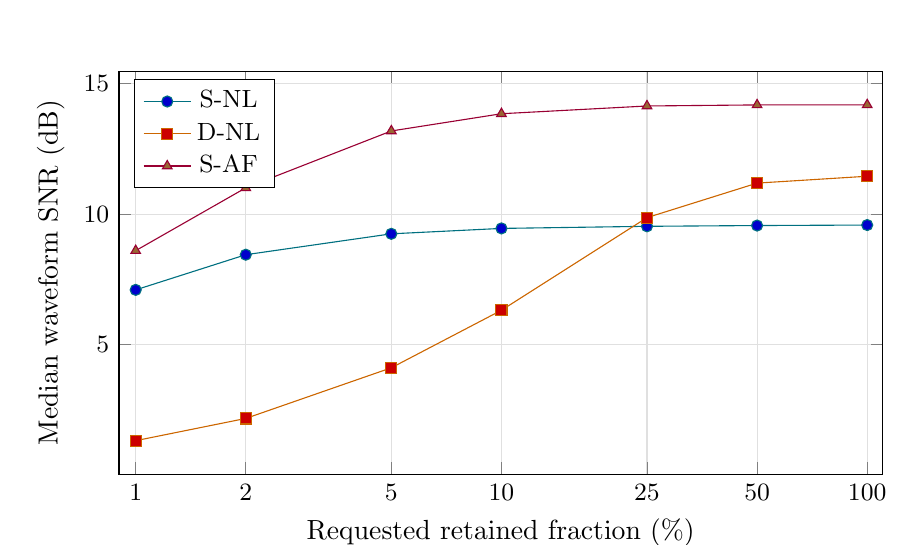
\begin{tikzpicture}
\begin{axis}[width=.93\linewidth,height=67mm,xmode=log,log basis x=10,xmin=.9,xmax=110,xtick={1,2,5,10,25,50,100},xticklabels={1,2,5,10,25,50,100},xlabel={Requested retained fraction (\%)},ylabel={Median waveform SNR (dB)},grid=both,minor grid style={black!5},major grid style={black!12},legend style={at={(.02,.98)},anchor=north west,font=\small},tick label style={font=\small}]
\addplot+[color=accent,mark=*] coordinates {(1,7.09601)(2,8.44383)(5,9.24446)(10,9.45182)(25,9.53240)(50,9.56204)(100,9.58066)};
\addlegendentry{S-NL}
\addplot+[color=orange!80!black,mark=square*] coordinates {(1,1.31588)(2,2.16833)(5,4.10971)(10,6.31505)(25,9.86492)(50,11.1883)(100,11.4515)};
\addlegendentry{D-NL}
\addplot+[color=purple!80!black,mark=triangle*] coordinates {(1,8.59972)(2,11.0067)(5,13.1869)(10,13.8476)(25,14.1445)(50,14.1853)(100,14.1890)};
\addlegendentry{S-AF}
\end{axis}
\end{tikzpicture}
\caption{Development reconstruction under common evaluation budgets. The horizontal axis is a requested fraction of valid latent capacity, not a measured bitrate. Lines join evaluated points and do not certify intermediate performance. The zero-code point is omitted from the logarithmic axis.}
\label{fig:curves}
\end{figure}

\subsection{Tolerance attainment}
\begin{center}
\begin{tabular}{lrrr}
\toprule
Target waveform NMSE & S-NL successes & D-NL successes & S-AF successes \\
\midrule
$\leq.1$ (SNR $\geq10$ dB) & 90/200 & 139/200 & 161/200 \\
$\leq.01$ (SNR $\geq20$ dB) & 0/200 & 2/200 & 18/200 \\
$\leq.001$ (SNR $\geq30$ dB) & 0/200 & 0/200 & 0/200 \\
\bottomrule
\end{tabular}
\end{center}
A success means \emph{some} point in the entire eight-budget sweep reaches the target; it does not imply success at the smallest budget. For the 10 dB target, median smallest tested support among successful recordings is 3,566.5 for S-NL, 39,296 for D-NL, and 2,438 for S-AF. These conditional medians use different successful subsets and varying recording lengths. They cannot by themselves establish a paired compression advantage. The success counts and full support--distortion curves must accompany them.

\subsection{What the observations currently support}
\begin{enumerate}
\item \textbf{Training through sparsification matters at low budgets.} At 1\%, S-NL's median SNR is 7.10 dB versus 1.32 dB for D-NL; at 10\%, it is 9.45 versus 6.32 dB. These are development observations from one seed, not general statistical conclusions.
\item \textbf{Dense quality and sparse robustness trade off.} At full support D-NL reaches 11.45 dB median SNR, above S-NL's 9.58 dB. The sparse model's early plateau shows that increasing the allowed support alone does not ensure near-accurate reconstruction.
\item \textbf{The affine control is a serious baseline.} S-AF reaches 13.85 dB median SNR at 10\% and 14.19 dB at full support, with better mean STOI/PESQ than both nonlinear models at these points. Greater network nonlinearity has not helped in this particular design and optimization budget. This does not prove affine representations are universally superior.
\item \textbf{The stated research goal remains open.} None of the three models reaches 30 dB SNR for any development utterance in the tested sweep. Neither low support nor favorable intelligibility demonstrates that all important details of the waveform have been preserved.
\end{enumerate}

\clearpage
\section{Held-out test-clean comparison}
The complete test uses all 2,620 recordings from 40 speakers, approximately 5.403 hours. None of these speakers occurs in the 921-speaker training set or 40-speaker development set. The checkpoint hashes, test-manifest hash, seed, eight fractions, and error thresholds were recorded before evaluation. All three checkpoints remain those previously selected at update 20,000; no retraining or test-driven model selection was performed.

Table~\ref{tab:test-results} is generated from the completed evaluation summaries. Mean and median conventions match the development table. Zero retained values are a reconstruction control, and do not imply that a nonzero STOI score demonstrates preserved speech information. The numeric export is \code{sparse_autoencoder_test_results.csv}; the frozen protocol and provenance are in \code{sparse_autoencoder_test_runs.json}.
\begin{table}[!htbp]
\centering\small
\begin{tabular}{llrrrrr}
\toprule
Model & Retained & Values/s & NMSE & SNR (dB) & STOI & PESQ-WB \\
\midrule
S-NL & 0\% & 0.0 & 1.0002 & -0.00 & 0.440 & 1.052 \\
S-NL & 1\% & 160.3 & 0.2597 & 6.89 & 0.705 & 1.255 \\
S-NL & 2\% & 320.6 & 0.2136 & 8.17 & 0.747 & 1.377 \\
S-NL & 5\% & 801.3 & 0.1892 & 9.06 & 0.779 & 1.518 \\
S-NL & 10\% & 1,602.5 & 0.1830 & 9.30 & 0.791 & 1.589 \\
S-NL & 25\% & 4,006.1 & 0.1799 & 9.42 & 0.800 & 1.645 \\
S-NL & 50\% & 8,012.1 & 0.1793 & 9.45 & 0.804 & 1.672 \\
S-NL & 100\% & 16,024.2 & 0.1792 & 9.45 & 0.806 & 1.680 \\
\midrule
D-NL & 0\% & 0.0 & 1.0170 & -0.05 & 0.423 & 1.038 \\
D-NL & 1\% & 160.3 & 0.7504 & 1.26 & 0.474 & 1.035 \\
D-NL & 2\% & 320.6 & 0.6243 & 2.09 & 0.517 & 1.041 \\
D-NL & 5\% & 801.3 & 0.4247 & 3.91 & 0.603 & 1.065 \\
D-NL & 10\% & 1,602.5 & 0.2801 & 6.09 & 0.688 & 1.119 \\
D-NL & 25\% & 4,006.1 & 0.1608 & 9.59 & 0.798 & 1.368 \\
D-NL & 50\% & 8,012.1 & 0.1340 & 10.92 & 0.849 & 1.780 \\
D-NL & 100\% & 16,024.2 & 0.1298 & 11.14 & 0.866 & 1.920 \\
\midrule
S-AF & 0\% & 0.0 & 1.0000 & -0.00 & 0.429 & 1.069 \\
S-AF & 1\% & 160.3 & 0.1981 & 8.20 & 0.732 & 1.276 \\
S-AF & 2\% & 320.6 & 0.1433 & 10.44 & 0.796 & 1.471 \\
S-AF & 5\% & 801.3 & 0.1134 & 12.32 & 0.851 & 1.793 \\
S-AF & 10\% & 1,602.5 & 0.1065 & 12.86 & 0.873 & 2.027 \\
S-AF & 25\% & 4,006.1 & 0.1037 & 13.14 & 0.890 & 2.277 \\
S-AF & 50\% & 8,012.1 & 0.1032 & 13.18 & 0.897 & 2.416 \\
S-AF & 100\% & 16,024.2 & 0.1032 & 13.18 & 0.899 & 2.472 \\
\bottomrule
\end{tabular}
\caption{Full held-out test-clean: 2,620 utterances, 40 speakers. Values/s, NMSE, STOI, and PESQ-WB are utterance means; SNR is the utterance median. Retained is the requested fraction of valid latent capacity. All scores use frozen checkpoints previously selected on development data.}
\label{tab:test-results}
\end{table}


\begin{figure}[!htbp]
\centering
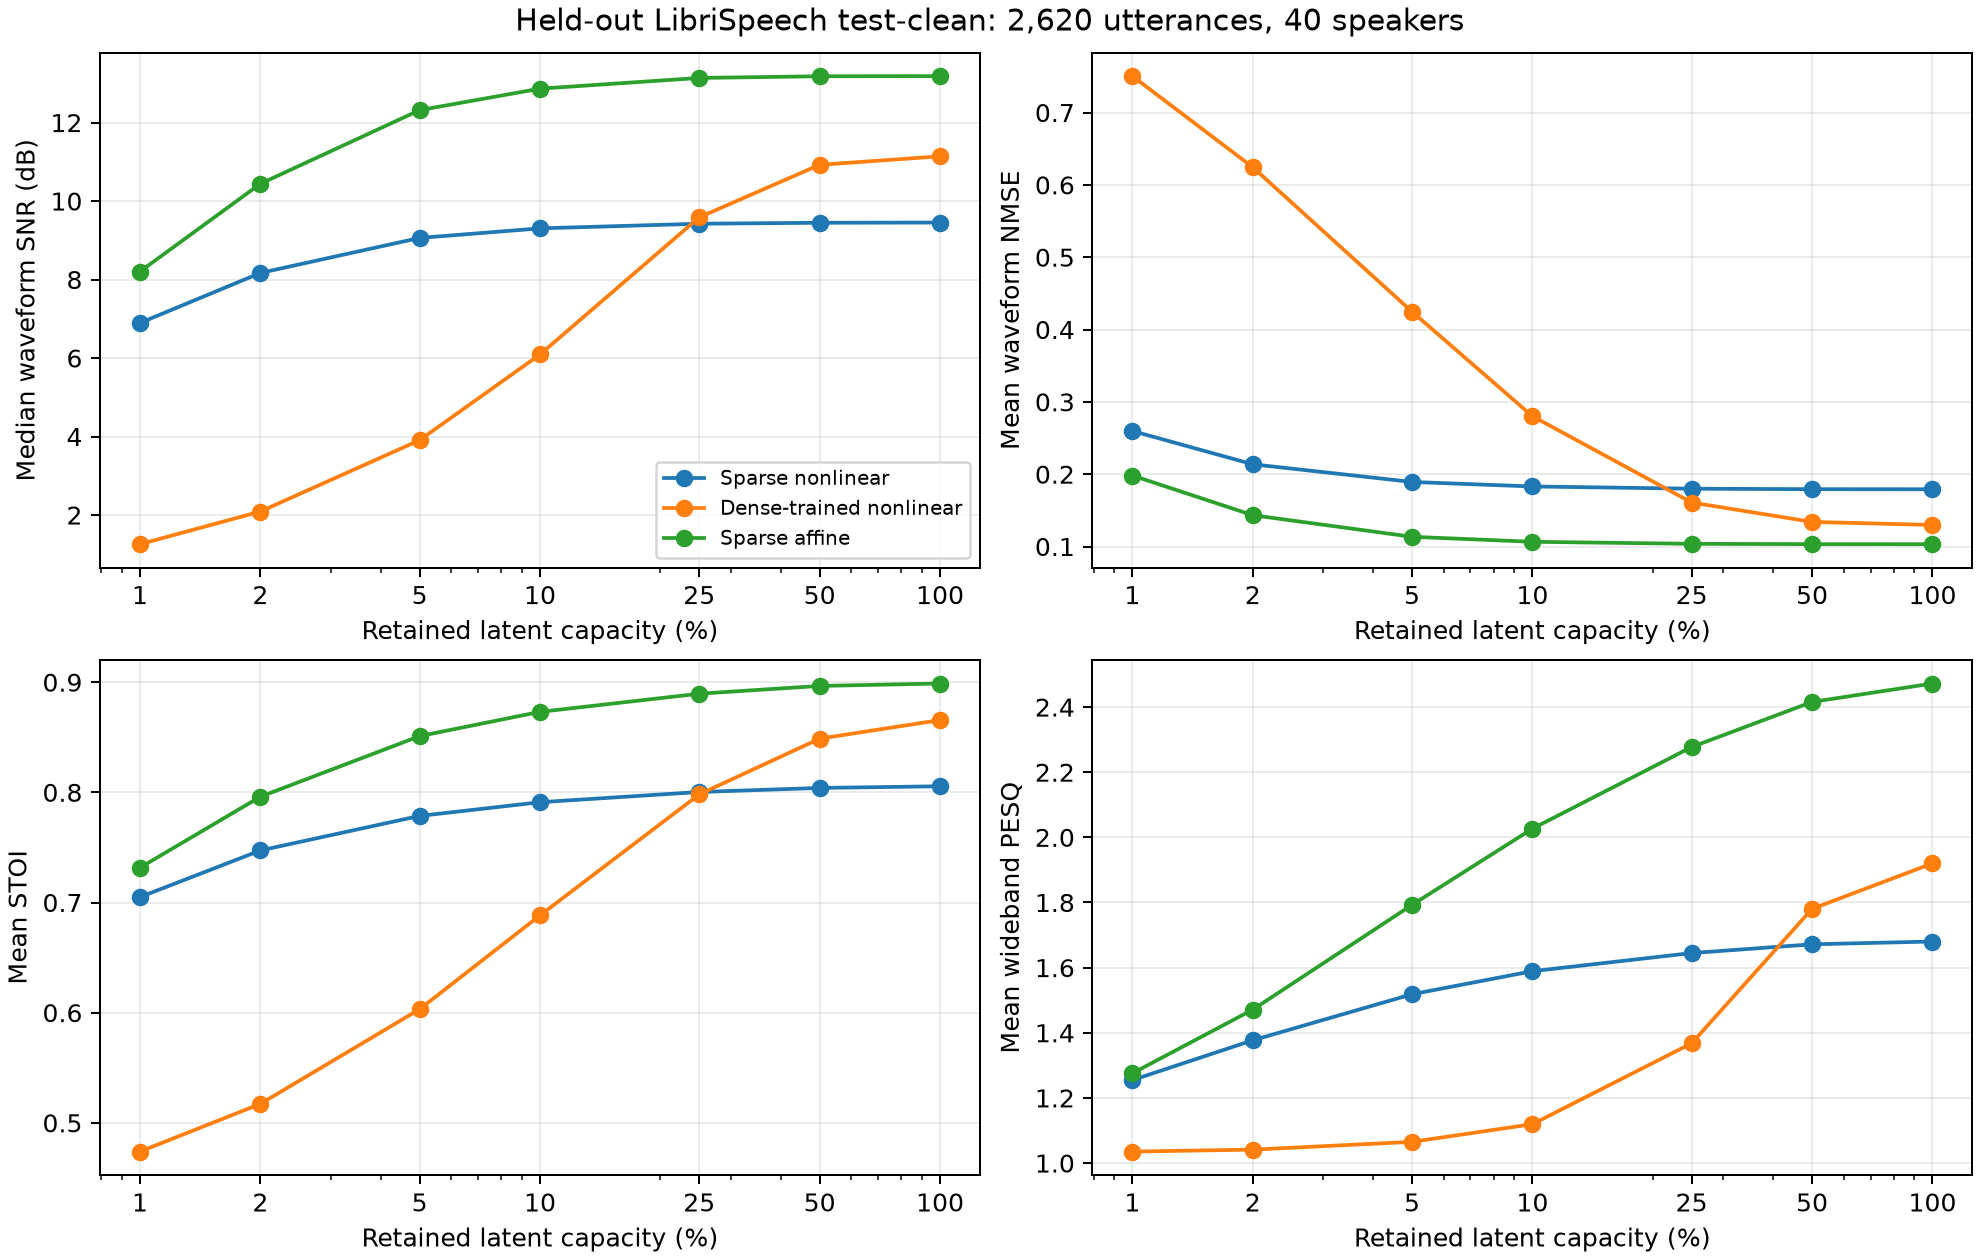
\includegraphics[width=\linewidth]{sparse_autoencoder_test_results.png}
\caption{Full held-out support--quality curves. Requested retained fraction is not a bitrate. The zero-code control is omitted from logarithmic axes. Curves summarize a fixed grid and do not establish intermediate or globally optimal performance.}
\end{figure}

\subsection{Interpreting the held-out findings}
At 1\% capacity, S-NL reaches 6.89 dB median SNR compared with D-NL's 1.26 dB. At 10\%, the values are 9.30 and 6.09 dB. Training through sparsification therefore improves low-budget robustness in this comparison. At full support, however, D-NL reaches 11.14 dB compared with S-NL's 9.45 dB. A representation trained to tolerate pruning need not offer the strongest dense reconstruction.

S-AF reaches 8.20 dB at 1\%, 12.86 dB at 10\%, and 13.18 dB at full support. At 10\%, its mean STOI is 0.873 and mean wideband PESQ is 2.027, compared with S-NL's 0.791 and 1.589. Its paired speaker-macro mean SNR advantage over S-NL is 3.52 dB, with a 95\% paired speaker-bootstrap interval of $[3.16,3.87]$ dB; its mean SNR difference is positive for all 40 speakers. This mean-difference interval is distinct from the difference between corpus medians.

\begin{center}
\begin{tabular}{lrrr}
\toprule
Target waveform NMSE & S-NL successes & D-NL successes & S-AF successes \\
\midrule
$\leq.1$ (SNR $\geq10$ dB) & 1,168/2,620 & 1,511/2,620 & 1,845/2,620 \\
$\leq.01$ (SNR $\geq20$ dB) & 0/2,620 & 1/2,620 & 105/2,620 \\
$\leq.001$ (SNR $\geq30$ dB) & 0/2,620 & 0/2,620 & 0/2,620 \\
\bottomrule
\end{tabular}
\end{center}
Each success permits any point in the frozen eight-budget sweep; these are not small-budget success counts. Among the 1,168 recordings where both S-AF and S-NL reach 10 dB, the median of their paired smallest-tested-support ratios $K_{\rm S\mbox{-}AF}/K_{\rm S\mbox{-}NL}$ is 0.50. S-AF uses strictly fewer retained values for 804 of those recordings and also succeeds on 677 recordings where S-NL fails. This supports an achieved representation-economy advantage for this comparison, while retaining the qualification that the supports come from a finite grid and a fixed inference rule.

The complete numerical comparison appears in the Markdown report, \path{sparse_autoencoder_test_results.md}. Its paired support analysis compares smallest tested supports on the \emph{same} recordings where both models meet a fixed error target. It reports the size of that common successful set alongside each conditional ratio. The paired JSON record, \path{sparse_autoencoder_test_paired.json}, also retains one-sided successes and failures. Different successful subsets must not be mistaken for a paired sparsity advantage.

The paired quality analysis resamples 40 speakers with 2,000 draws under seed 0, after averaging matched utterance differences within each speaker. Its 95\% percentile intervals concern speaker-macro \emph{mean differences}, not differences of median SNR or variability across training seeds. Per-budget summaries additionally retain the original 1,000-resample speaker intervals.

The hidden $H=N/2$ bottleneck identified in the architecture review materially limits interpretation of the full-budget floor. This experiment tests achieved sparse representations produced by three particular compressed encoder--decoder designs. It does not isolate sparsification from a lossless dense reference, and the affine rank bound does not by itself quantify the observed error for a particular speech signal. A subsequent experiment should first establish dense reconstruction fidelity, then measure the additional cost of sparsification under a controlled representation.

PESQ and STOI used CPU worker processes with the same metric functions and input arrays; a regression check confirmed equality with serial evaluation. GPU jobs were eventually scheduled sequentially after concurrent evaluation filled device memory. Earlier completed budgets were retained under the same frozen checkpoints and coverage. Resource scheduling and a larger CPU pool change execution time, not the reconstruction rule, metric definitions, or selected model. Timings are not used for architecture-speed conclusions.

\section{Reproduction, files, and code correspondence}
\subsection{Minimal workflow}
Use Python 3.11 or newer and a PyTorch build suitable for the machine. From the repository root, a fresh installation can use:
\begin{lstlisting}
python -m venv .venv
# Activate the environment for your shell, then:
python -m pip install -e ".[dev]"
# Optional, needed to reproduce PESQ/STOI columns:
python -m pip install -e ".[speech-metrics]"
\end{lstlisting}
Native compilation may be required for the optional PESQ package. The version snapshot in \code{requirements-lock.txt} records the workstation environment; its CUDA-wheel availability is platform-dependent.

Set \code{data.root} in \code{configs/data_librispeech_cached.yaml} to the local corpus/cache root. Official payloads are available at \url{https://www.openslr.org/12}. Both standard \code{LibriSpeech/<partition>} layout and Kaggle's \code{<partition>/LibriSpeech/<partition>} layout are supported. Do not substitute a single-speaker corpus under the same configuration. Prepare once:
\begin{lstlisting}
python run.py prepare --config configs/librispeech_sparse_autoencoder_10h.yaml
python run.py audit --config configs/librispeech_sparse_autoencoder_10h.yaml
\end{lstlisting}
Then run each experiment, reusing manifests:
\begin{lstlisting}
python run.py experiment --config configs/librispeech_sparse_autoencoder_10h.yaml --skip-prepare
python run.py experiment --config configs/librispeech_sparse_autoencoder_dense_10h.yaml --skip-prepare
python run.py experiment --config configs/librispeech_sparse_autoencoder_affine_10h.yaml --skip-prepare
\end{lstlisting}
These commands prepare no additional speech download, train, evaluate the development probe, analyze a bounded subset, and write a report in the printed run directory. Running sequentially is sufficient; concurrency is not part of the scientific model definition.

For a saved run, an explicit development sweep is
\begin{lstlisting}
python run.py evaluate --run runs/YOUR_RUN --split validation --limit 200 --keep-fractions 0,0.01,0.02,0.05,0.1,0.25,0.5,1
\end{lstlisting}
The held-out test in this revision uses \code{--split clean} without a development limit. Optional \code{--metric-workers 4} parallelizes CPU PESQ/STOI calculations. \code{--resume} reuses completed budgets with matching coverage and checkpoint metadata; the frozen study additionally verifies checkpoint and manifest hashes. \code{python tools/compare_models.py} regenerates the test comparison, paired support/quality analysis, figure, and numeric exports from completed local runs.

The evaluator loads \code{checkpoints/best.pt} by default. Checkpoints contain model/optimizer states, configuration, training power, update count, and stored RNG state. Training resume restores model/optimizer RNG but restarts the crop/sampler position; an interrupted/resumed training trajectory is not promised to match an uninterrupted one bit for bit. GPU numerical kernels can also limit exact cross-machine reproduction.

\subsection{Implementation map}
\begin{center}\small
\begin{tabularx}{\linewidth}{lY}
\toprule
Source & Responsibility \\
\midrule
\code{lrac/models/autoencoder.py} & Convolutional stages, residual blocks, decoder ordering \\
\code{lrac/models/sparse_autoencoder.py} & Length-safe encoding, global top-$k$, identity activation control \\
\code{lrac/train.py} & Sampling, objective, AdamW, validation, checkpoint selection \\
\code{lrac/losses.py} & Masked MSE and spectral diagnostics \\
\code{lrac/metrics.py} & Waveform/STFT/speech metrics, speaker bootstrap \\
\code{lrac/evaluate.py} & Budget sweep, support counts, tested-support search \\
\code{lrac/data/datasets.py} & Speaker coverage, weighted sampling, crops, collation \\
\code{lrac/data/manifests.py} & Deterministic subset construction and corpus indexing \\
\code{lrac/data/audit.py} & Roles, speakers, source intervals, duplicate-hash audit \\
\code{tests/test_sparse_autoencoder.py} & Shapes, padding, code-only decode, gradients, affine control \\
\bottomrule
\end{tabularx}\end{center}
The existing suite also exercises audits, metric validity, dataset sampling, checkpoint reuse, and the end-to-end workflow. All 62 tests passed during this revision, including process-worker metric equality and reuse of completed evaluation budgets. Documentation and exported results do not replace the executable implementation.

The repository includes the \LaTeX{} source, BibTeX references, compiled PDF, a numeric results export, and a compact run/provenance record. Downloaded recordings, generated path-bearing manifests, environments, checkpoints, and bulky run products are excluded by \code{.gitignore}. Retraining regenerates local run artifacts; published scalar results alone do not provide downloadable pretrained models.

To rebuild this document from \code{documentation/}, with a \LaTeX{} distribution including BibTeX, TikZ, and PGFPlots:
\begin{lstlisting}
latexmk -pdf -interaction=nonstopmode -halt-on-error sparse_autoencoder_models.tex
\end{lstlisting}

\section{Limits and next research decisions}
\subsection{What the baseline does not establish}
\begin{itemize}
\item \textbf{Global sparsestness:} encoder inference and magnitude top-$k$ do not solve Eq.~\eqref{eq:ideal} over arbitrary decoders or even all codes for the trained decoder. General fixed-dictionary sparse approximation is already computationally difficult~\cite{natarajan1995}; that result does not prove an impossibility theorem for every restricted neural formulation.
\item \textbf{Exact reconstruction or invertibility:} no Jacobian, frame-bound, or perfect-reconstruction constraint is enforced. Full-budget residual error is substantial.
\item \textbf{Per-sample optimal adaptation:} the learned bank of convolutional parameters is shared. Only latent values and positions adapt. There is no search over input-dependent transforms, learned stopping rule, per-example latent optimization, or certified lower bound.
\item \textbf{Bitrate and arbitrary precision:} values remain float32 and no entropy-coded bitstream is produced. A one-number code with unbounded numerical precision would be an accounting loophole, not evidence of physical compression.
\item \textbf{General audio generalization:} the main data are clean English read speech and one training seed. Full held-out \code{test-clean} evaluation checks unseen narrators in this corpus; it does not establish transfer to all signals.
\item \textbf{Semantic or independent features:} a coordinate is an operational reconstruction variable. Neither semantic interpretation, orthogonality, nor independence is required or demonstrated.
\end{itemize}

\subsection{Questions made sharper by the three runs}
The first priority is to explain the full-budget reconstruction floor before treating sparse quality as a fundamental limit. Useful controlled tests would vary downsampling/receptive field, initialization, training duration, and waveform versus spectral objectives while retaining common data and checkpoint criteria. The current affine advantage motivates a simple perfect-reconstruction or invertible analysis--synthesis reference rather than assuming that additional nonlinear depth is the answer.

Next, compare hard magnitude ranking with reconstruction-aware support refinement under a \emph{fixed} decoder and fixed budget. For S-AF, optimize selected coefficients and test alternative supports; for S-NL, separate amplitude optimization from support changes. Any gains would quantify the inference gap between this encoder and better codes within the same decoder, without conflating that gap with model capacity. Analyze paired recordings at matched distortion and report failures as well as successes.

Finally, repeat with multiple seeds and develop subsequent architectures on training/development data. This test-clean result is now a fixed baseline; further test-driven choices should not be presented as fresh independent confirmation. Synthetic signals remain useful because known generative structure can expose failures, but success on selected synthetic families would not establish universality. Quantization, support coding, and shared-model accounting should be added when comparing actual description lengths. These questions keep the experiment connected to the dream system while avoiding claims the current evidence cannot support.

\bibliographystyle{unsrtnat}
\bibliography{sparse_autoencoder_models}
\end{document}
